\chapter{Diseño}

\section{Introducción}
En este capítulo se realizará el diseño del software a desarrollar. Para ello, se detallará cómo se va a desarrollar la aplicación, qué arquitectura y tecnologías se van a utilizar y cómo se va a realizar el diseño de la interfaz de usuario. 
Esta fase tiene como objetivo definir la estructura del sistema y la función de cada una de sus partes, lo cual permitirá que el desarrollo sea más eficiente y que el resultado final tenga mayor calidad.

\section{Arquitectura del sistema}
Para el desarrollo de la aplicación se ha decidido utilizar una arquitectura \textbf{cliente-servidor}, donde el servidor será responsable de las operaciones relacionadas con la gestión (añadir, extraer, eliminar y/o modificar) de la información almacenada en la base de datos, mientras que el cliente será 
la aplicación móvil que se encargará de mostrar la información al usuario y de realizar las operaciones que el usuario solicite. Además, también será una arquitectura basada en el patrón de diseño \textbf{Modelo / Vista / Controlador (MVC)}, donde el modelo gestionará y mantendrá la estructura de la información
de la base de datos, la vista se hará cargo de mostrar la información al usuario y facilitar la interacción de este con el sistema y el controlador se encargará de gestionar las operaciones que el usuario solicite. Todo esto mediante las tecnologías \textbf{Node.js} para el controlador, \textbf{Mongoose} para
el modelo, \textbf{MongoDB} para la base de datos y \textbf{Flutter} para las distintas vistas que los usuarios tendrán. 

\begin{figure}[H]
    \centering
    \centerline{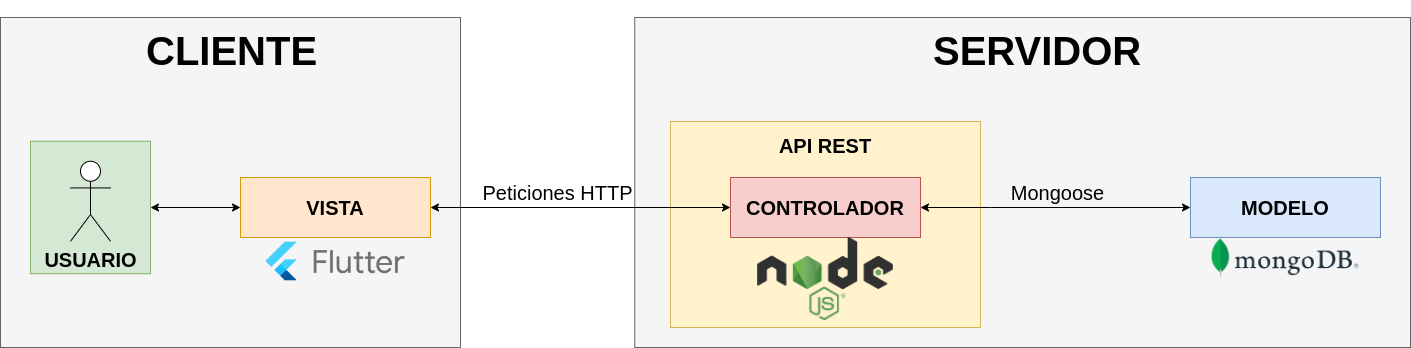
\includegraphics[width=1.1\textwidth]{imagenes/c6/arch.png}}
    \caption{Diagrama de la arquitectura del sistema, donde se muestra la comunicación entre el servidor y la aplicación móvil.}
    \label{fig:diagramadearquitectura}    
\end{figure}

Como podemos ver en el diagrama, el controlador tendrá una API REST que será la encargada de gestionar las peticiones que se realicen desde la aplicación móvil. La API REST es una interfaz que permite la comunicación entre dos sistemas de computación (en nuestro caso, entre el cliente y el servidor) para
el intercambio de información de manera segura. REST definirá las restricciones a cumplir dentro de nuestra arquitectura, como por ejemplo la necesidad de utilizar los principales verbos HTTP (GET, POST, PUT y DELETE) para realizar las operaciones de lectura, creación, actualización y eliminación de la información.

\section{Diagrama de base de datos}
En cuanto al diagrama de base de datos, se ha realizado un diagrama de base de datos no relacional, que representa los distintos documentos 
que tendrá nuestra base de datos de MongoDB. En este caso, se han definido 5 documentos, uno para los usuarios, otro para las lecciones, otro para los tests, otro para las preguntas de los tests y otro para
los logros. También se han definido las referencias que habrá entre los documentos, como por ejemplo que un usuario tiene varios logros.

\begin{figure}[H]
    \centering
    \centerline{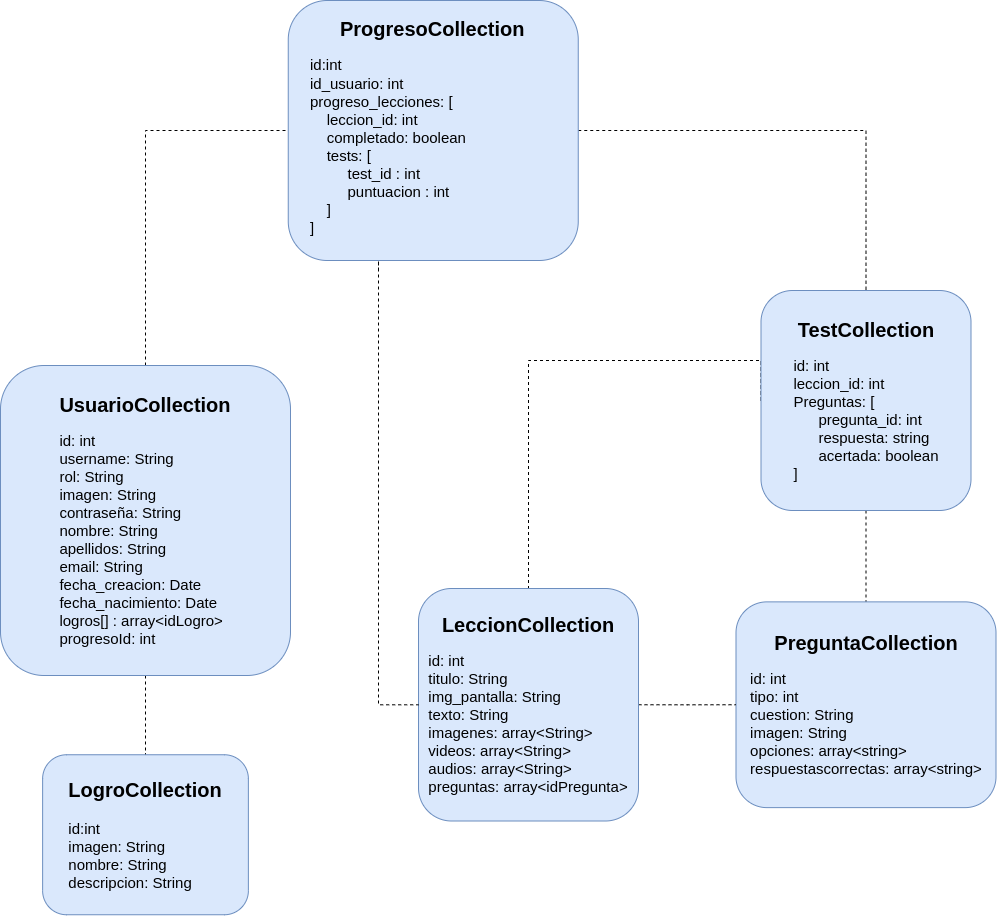
\includegraphics[width=\textwidth]{imagenes/c6/bbdd.png}}
    \caption{Diagrama de base de datos del sistema, donde se muestran los documentos que se van a almacenar en nuestra base de datos de MongoDB.}
    \label{fig:diagramadearquitectura}    
\end{figure}

En el diagrama se pueden ver varias referencias entre las colecciones de datos que se explicarán a continuación:
\begin{itemize}
    \item Un usuario tendrá los logros que consiga al progresar en la aplicación.
    \item Un usuario tiene un progreso, que contendrá las lecciones que realice junto con los tests que haya contestado.
    \item Un test tendrá varias preguntas (alrededor de 10) y estas se generarán de forma aleatoria cuando se cree el test.
    \item Una lección tendrá varias preguntas y de dicho conjunto de preguntas se seleccionarán algunas al azar para formar el test.
    \item Un test pertenecerá a una lección: un test solo podrá pertenecer a una lección (aquella donde se generó dicho test).
\end{itemize}

\section{Diagrama de clases}
A continuación se muestra el diagrama de clases de diseño, el cual se ha realizado a partir del diagrama de clases de análisis del capítulo anterior En esta ocasión se han detallado más
los atributos y los métodos de cada clase, facilitando así la comprensión de las relaciones entre las clases y de la estructura del sistema.
\begin{figure}[H]
    \centering
    \centerline{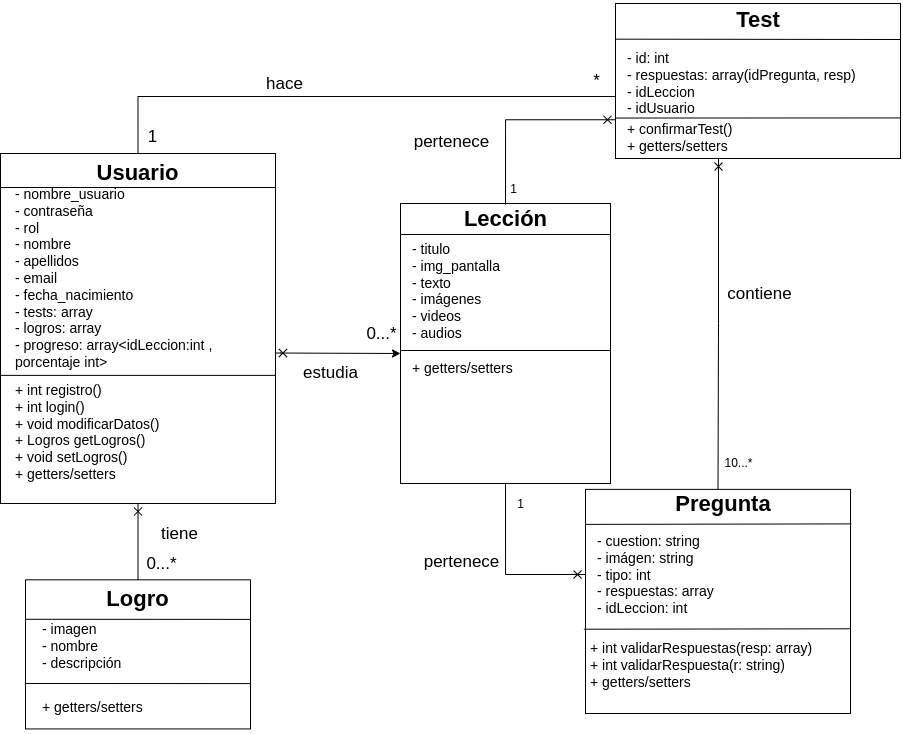
\includegraphics[width=\textwidth]{imagenes/c6/diagramadeclases.png}}
    \caption{Diagrama de clases del sistema donde se detallan las propiedades y las relaciones de las distintas clases o entidades que tendrá el software.}
    \label{fig:diagramadearquitectura}    
\end{figure}

\section{Diagramas de secuencia}
En lo que respecta a los diagramas de secuencia, se han realizado algunos ejemplos de cómo sería el flujo de una operación en el sistema. Como hemos visto anteriormente,
se seguirá una arquitectura basada en el patrón de diseño MVC, por lo que las peticiones pasarán por la vista, luego por el controlador y finalmente por el modelo.
En este caso, se ha realizado un diagrama de secuencia de cómo sería el flujo de una operación en la que un usuario se registra en la aplicación, otro para un usuario que contesta un test y otro
para un profesor que modifica una lección.

\begin{figure}[H]
    \centering
    \centerline{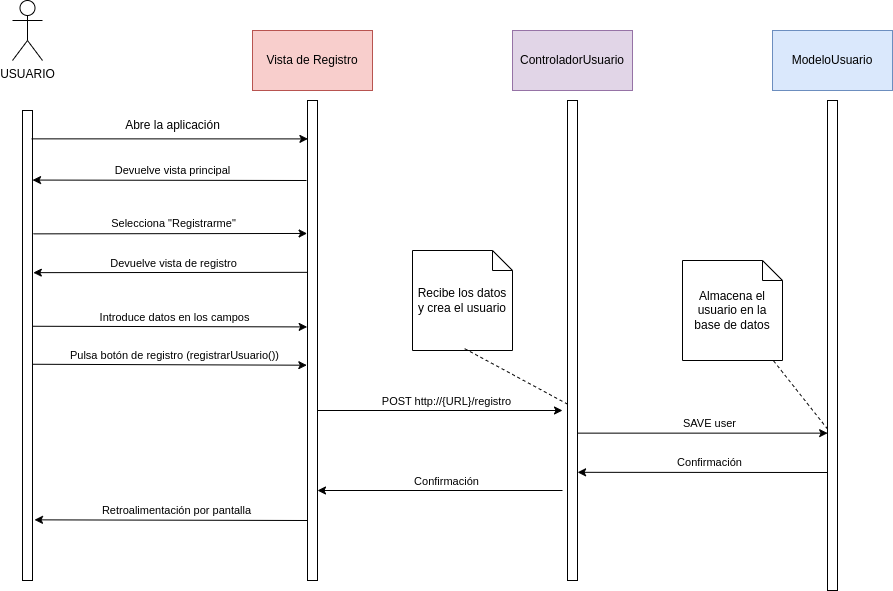
\includegraphics[width=\textwidth]{imagenes/c6/diagramadesecuencia.png}}
    \caption{Diagrama de secuencia de un usuario registrandose, el cual interactuará con la vista para poder hacer la petición al controlador y guardar su usuario en el modelo.}
    \label{fig:diagramadesecuencia}    
\end{figure}

\begin{figure}[H]
    \centering
    \centerline{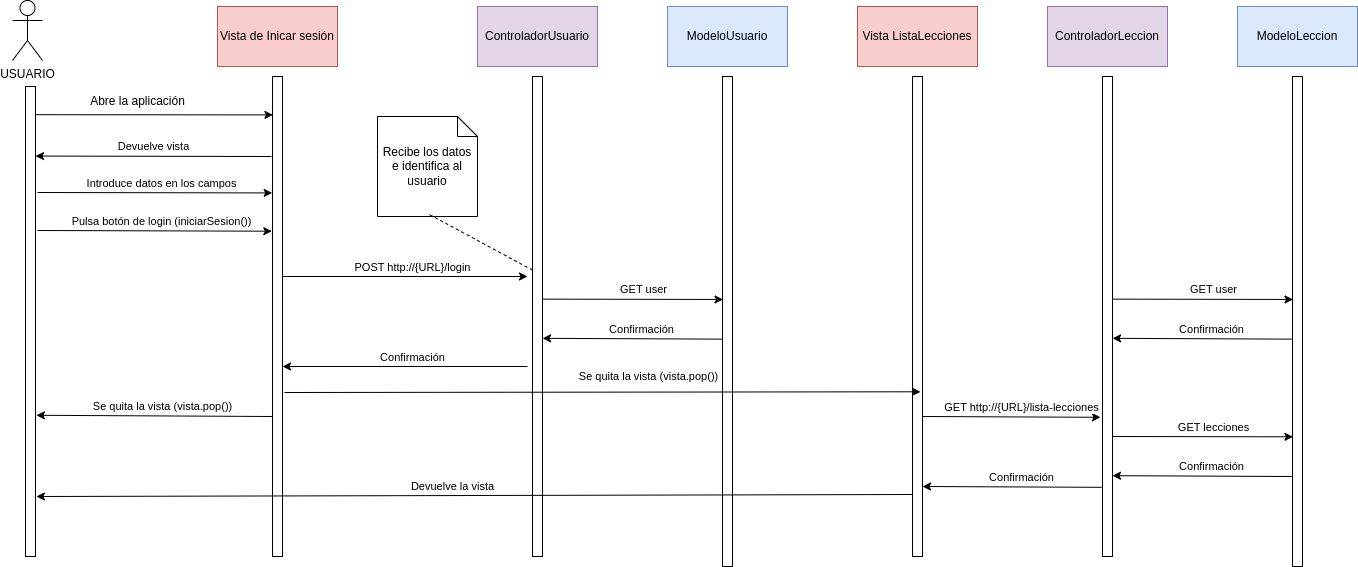
\includegraphics[width=\textwidth]{imagenes/c6/diagramadesecuencia2.png}}
    \caption{Diagrama de secuencia de un usuario iniciando sesión, el cual interactuará con la vista para poder hacer la petición al controlador y buscar su usuario en el modelo para la validación. Tras esto, se cambiará la vista a la pantalla principal que lista las lecciones, por lo que la vista deberá hacer otra petición al controlador de lecciones para obtener las lecciones del modelo.}
    \label{fig:diagramadesecuencia}    
\end{figure}

\newpage
\section{Diseño de interfaces de usuario}
Por último, en este apartado se presentan los bocetos de las interfaces de usuario que se han diseñado para la aplicación. Estos bocetos se han realizado con la herramienta Canva y serán de ayuda para la realización del diseño final de las interfaces de usuario,
que, pese a que seguirán una estructura similar a la de los bocetos, podrán variar en algunos detalles y aspectos de diseño.
\\

\subsection*{Inicio de sesión}

Esta vista se mostrará al usuario cuando inicie la aplicación y no tenga la sesión iniciada. En ella se pedirá al usuario que introduzca su correo electrónico y su contraseña para poder iniciar sesión en la aplicación. Si el usuario no tiene una cuenta, podrá pulsar en el botón de registro para poder crear una nueva cuenta.

\begin{figure}[H]
    \centering
    \centerline{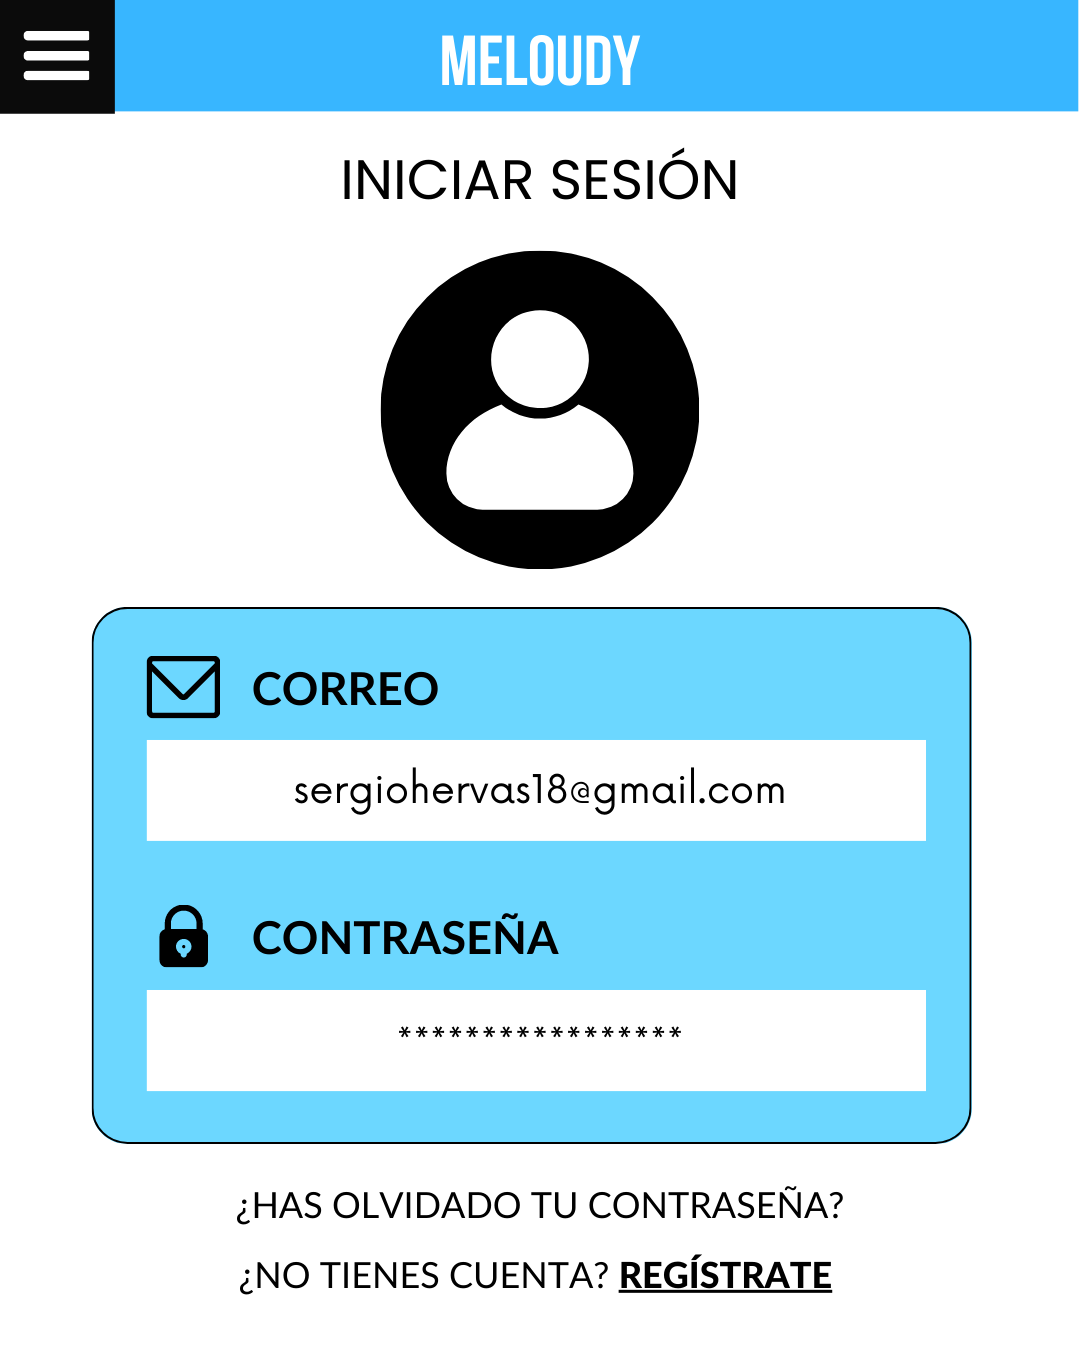
\includegraphics[width=0.45\textwidth, frame]{imagenes/c6/9.png}}
    \caption{Boceto de la pantalla de inicio de sesión, donde se pedirá al usuario el correo electrónico y la contraseña.}
    \label{fig:login}
\end{figure}


\subsection*{Registro}

Esta vista se mostrará al usuario cuando pulse en el botón de registro de la pantalla de inicio de sesión. En ella se pedirá al usuario que introduzca sus datos personales para poder crear una nueva cuenta en la aplicación. Si el usuario ya tiene una cuenta, podrá pulsar en el botón de inicio de sesión para poder iniciar sesión en la aplicación.

\begin{figure}[H]
    \centering
    \centerline{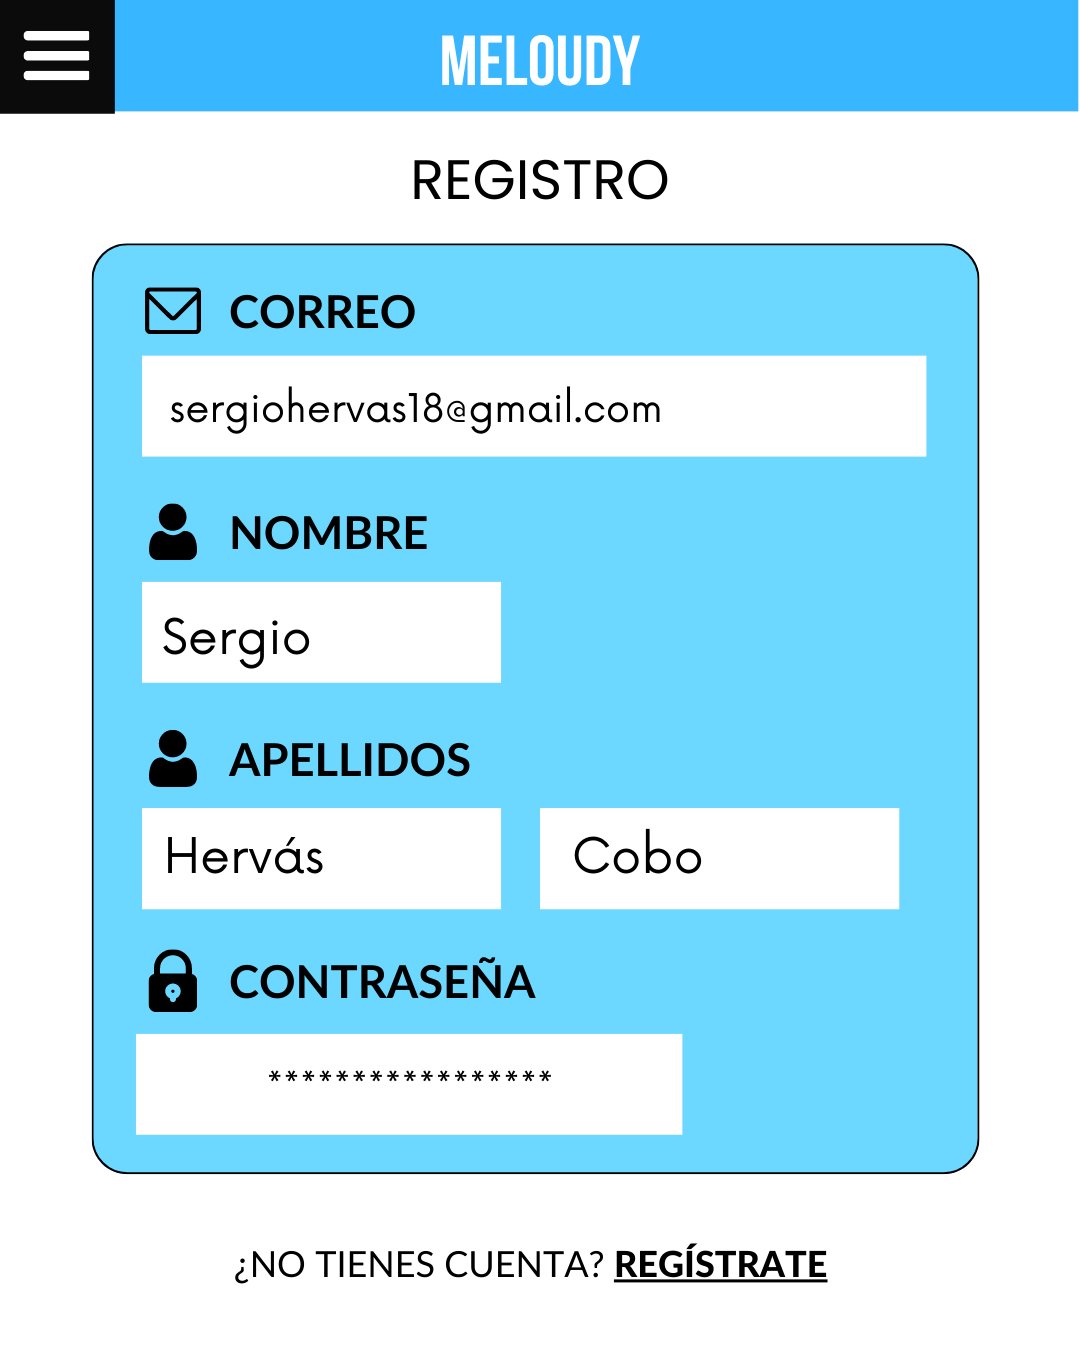
\includegraphics[width=0.45\textwidth, frame]{imagenes/c6/10.png}}
    \caption{Boceto de la pantalla de registro, donde se pedirá al usuario sus datos personales necesarios para crear la cuenta como el nombre, los apellidos, el correo y la contraseña.}
    \label{fig:registro}
\end{figure}


\subsection*{Lista de lecciones}

Esta vista se mostrará al usuario cuando inicie la aplicación y tenga la sesión iniciada. En ella se mostrarán las lecciones disponibles para el usuario y podrá seleccionar una de ellas para poder acceder a su contenido.

\begin{figure}[H]
    \centering
    \centerline{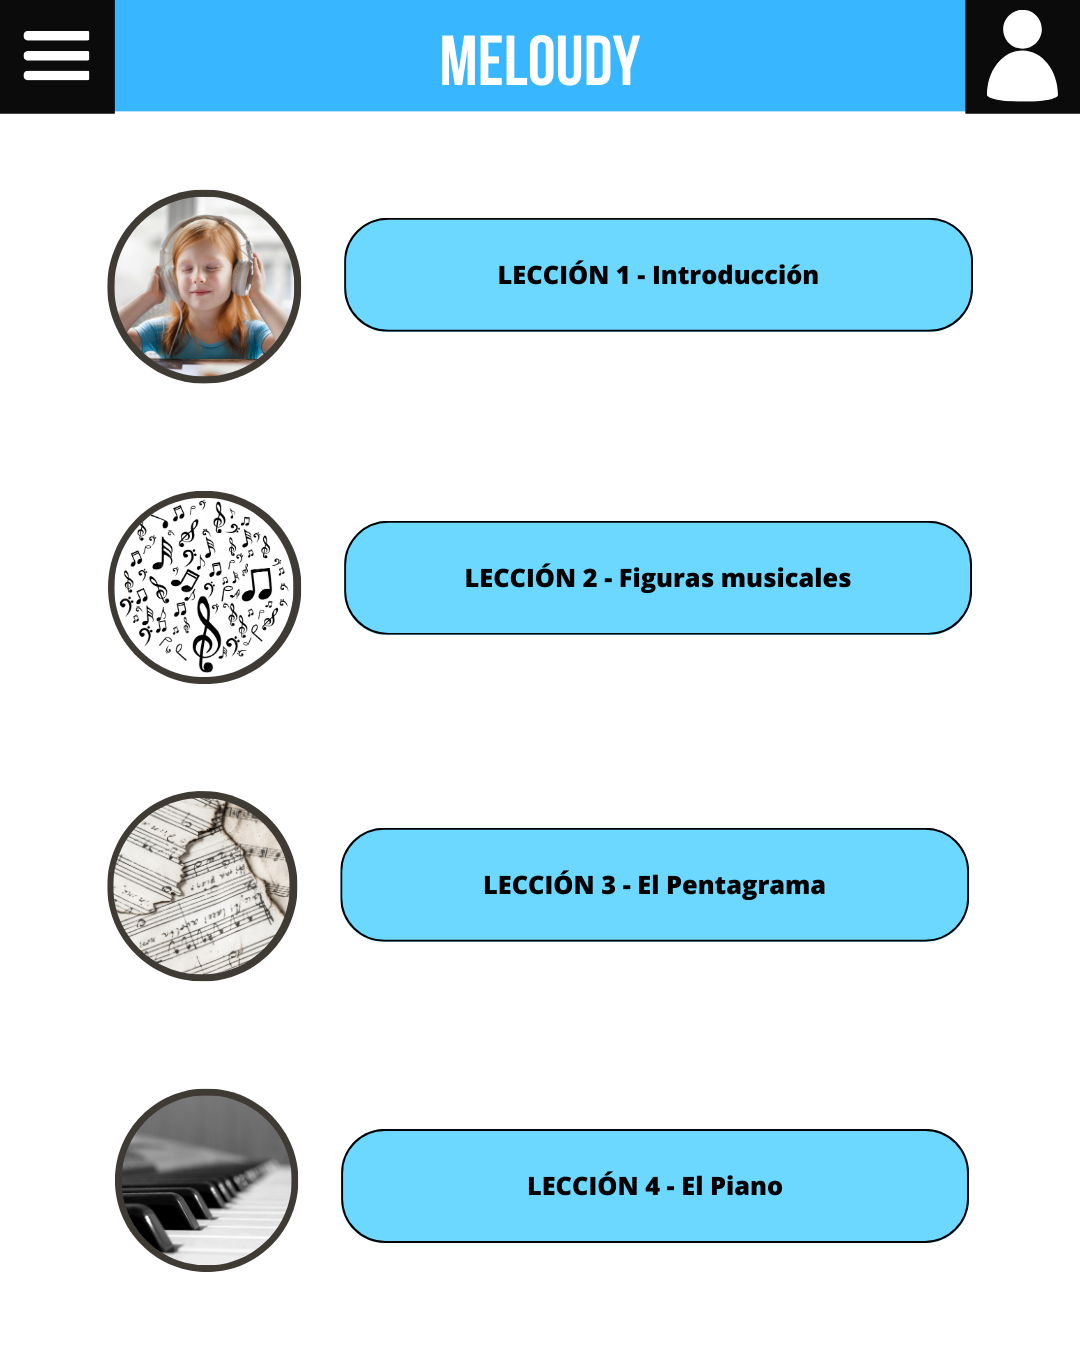
\includegraphics[width=0.45\textwidth, frame]{imagenes/c6/1.png}}
    \caption{Boceto de la pantalla principal de la aplicación donde se muestran las lecciones disponibles para el usuario.}
    \label{fig:pantallaprincipal}
\end{figure}


\subsection*{Perfil de usuario}

Esta vista se mostrará al usuario cuando pulse en el botón de perfil de la pantalla principal de la aplicación. En ella se mostrarán los datos del usuario y podrá acceder a sus logros y a la modificación de sus datos.
\begin{figure}[H]
    \centering
    \centerline{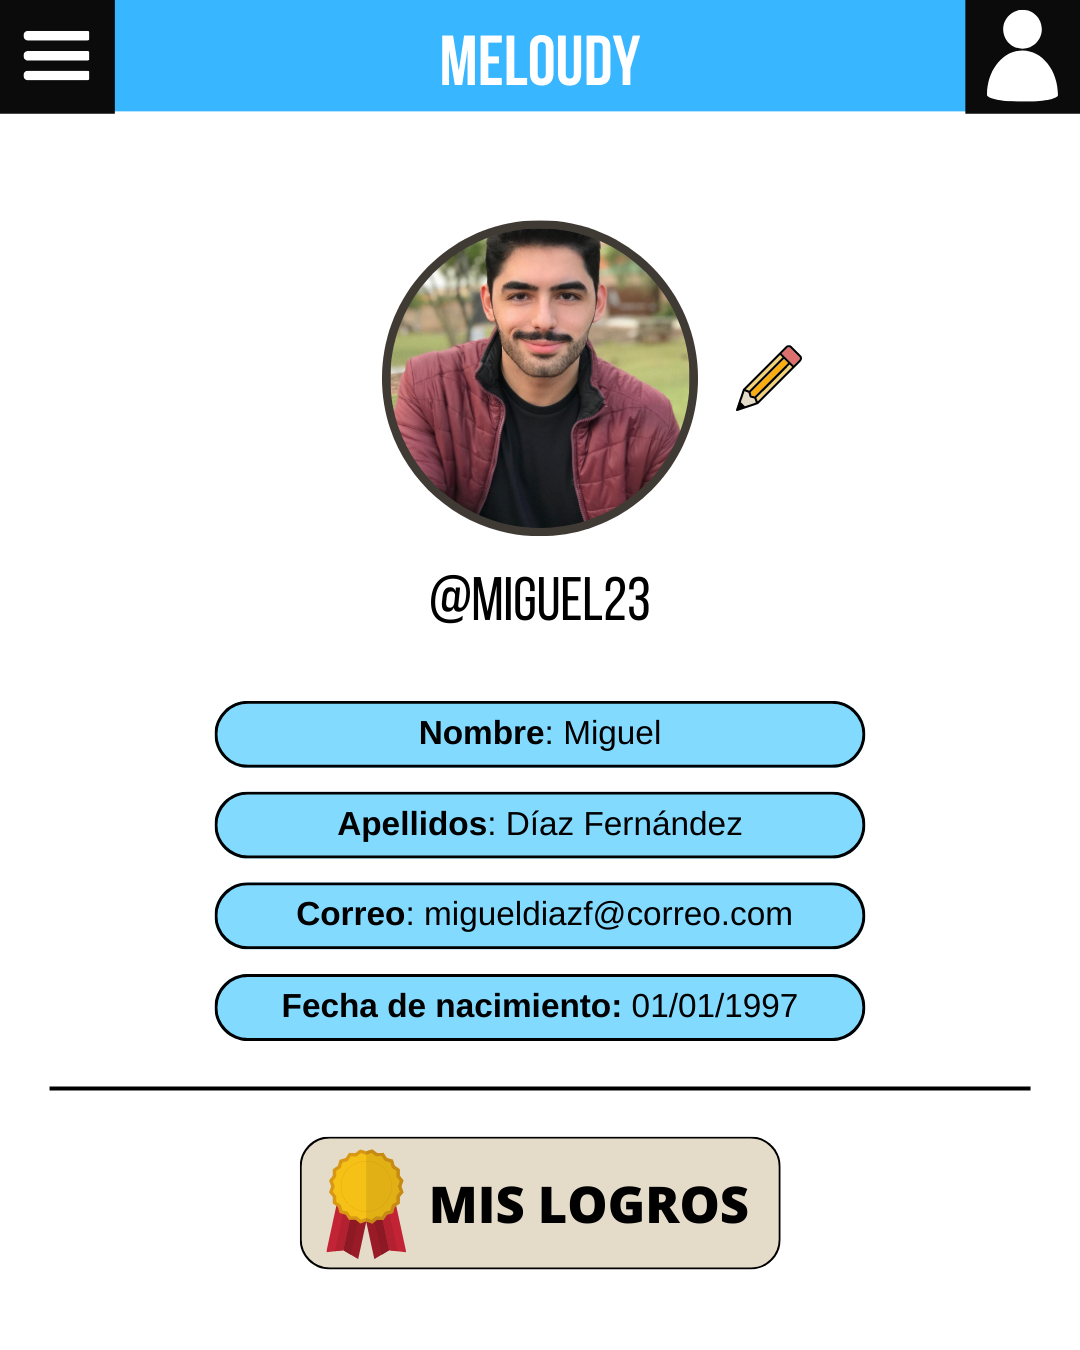
\includegraphics[width=0.40\textwidth, frame]{imagenes/c6/2.png}}
    \caption{Boceto de la pantalla del perfil de usuario con sus datos.}
    \label{fig:perfil}
\end{figure}

\subsection*{Lista de logros}

Esta vista se mostrará al usuario cuando pulse en el botón de logros de la pantalla del perfil de usuario. En ella se mostrarán los logros conseguidos por el usuario. Pulsando en cada logro se mostrará el nombre y la descripción de este.
\begin{figure}[H]
    \centering
    \centerline{
\includegraphics[width=0.40\textwidth, frame]{imagenes/c6/3.png}}
    \caption{Boceto de la pantalla de logros conseguidos por el usuario.}
    \label{fig:logros}
\end{figure}

\subsection*{Lección}

Esta vista se mostrará al usuario cuando pulse en una lección de la pantalla principal de la aplicación. En ella se mostrará el texto de la lección, el contenido multimedia y el botón para comenzar el test.

\begin{figure}[H]
    \centering
    \centerline{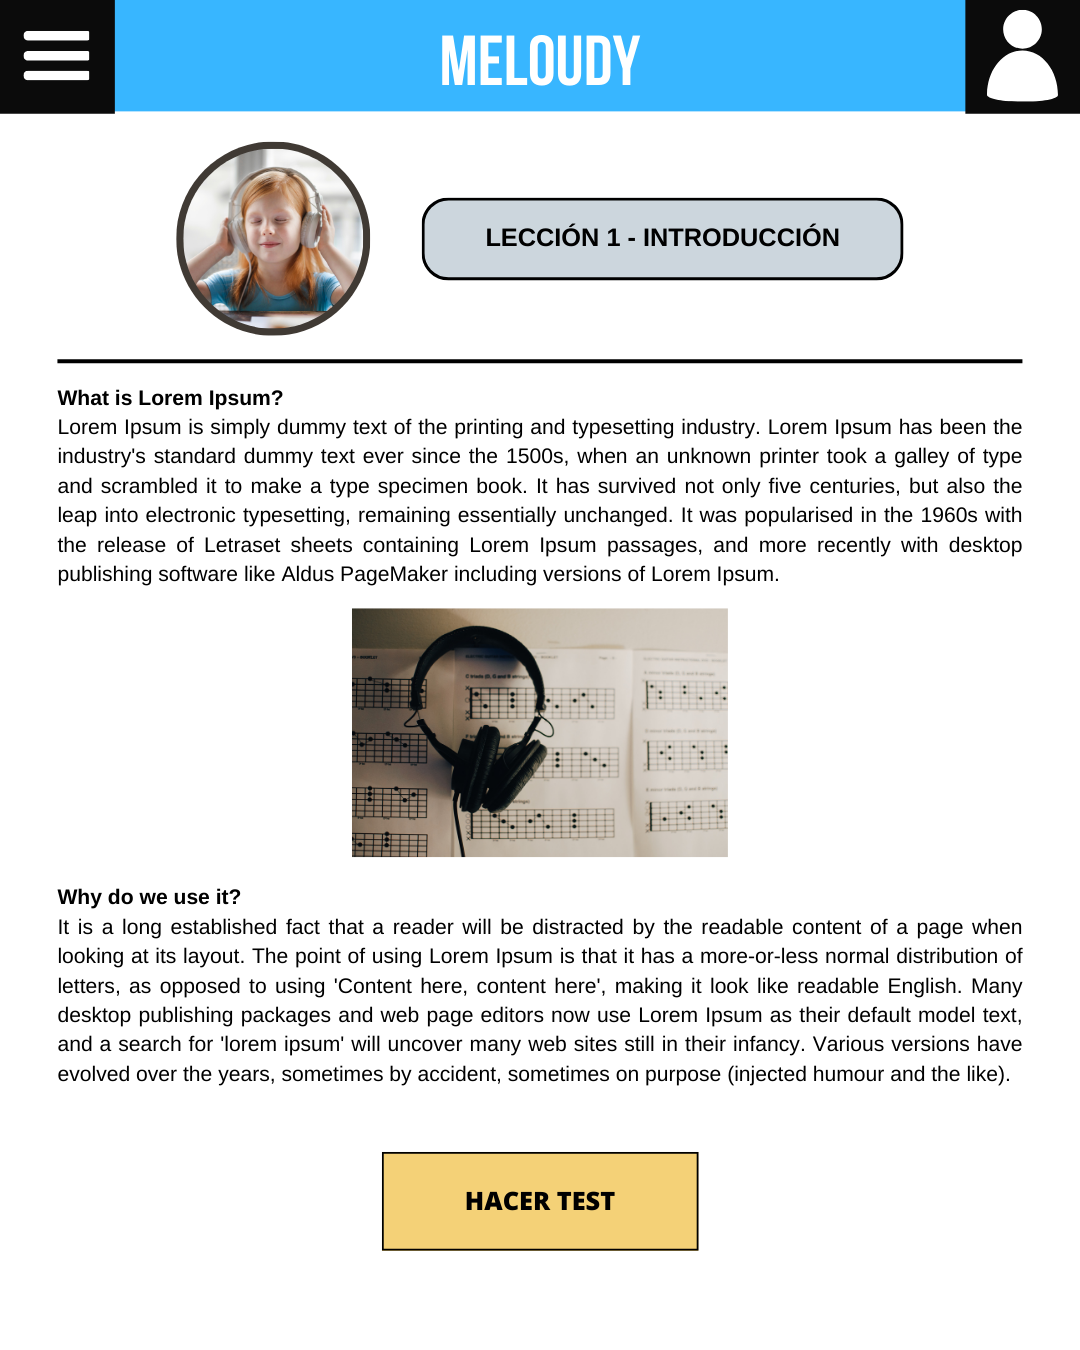
\includegraphics[width=0.45\textwidth, frame]{imagenes/c6/4.png}}
    \caption{Boceto de la pantalla de una lección, con el texto, el contenido multimedia y el botón para comenzar el test.}
    \label{fig:leccion}
\end{figure}

\newpage

\subsection*{Pregunta de selección única}

Con esta vista se mostrará al usuario una pregunta de test de tipo selección única. En ella se mostrará la pregunta y las opciones de respuesta. El usuario podrá seleccionar solamente una de ellas y pulsar en el botón de comprobar para comprobar si la respuesta es correcta o no. Si la respuesta es correcta, se mostrará un mensaje de felicitación y se mostrará el botón de siguiente para pasar a la siguiente pregunta. Si la respuesta es incorrecta, se mostrará un mensaje de error y se mostrará el botón de siguiente para pasar a la siguiente pregunta. Si el usuario no ha seleccionado ninguna opción, se mostrará un mensaje de error y no se podrá pasar a la siguiente pregunta hasta que no seleccione una opción.


\begin{figure}[H]
    \centering
    \centerline{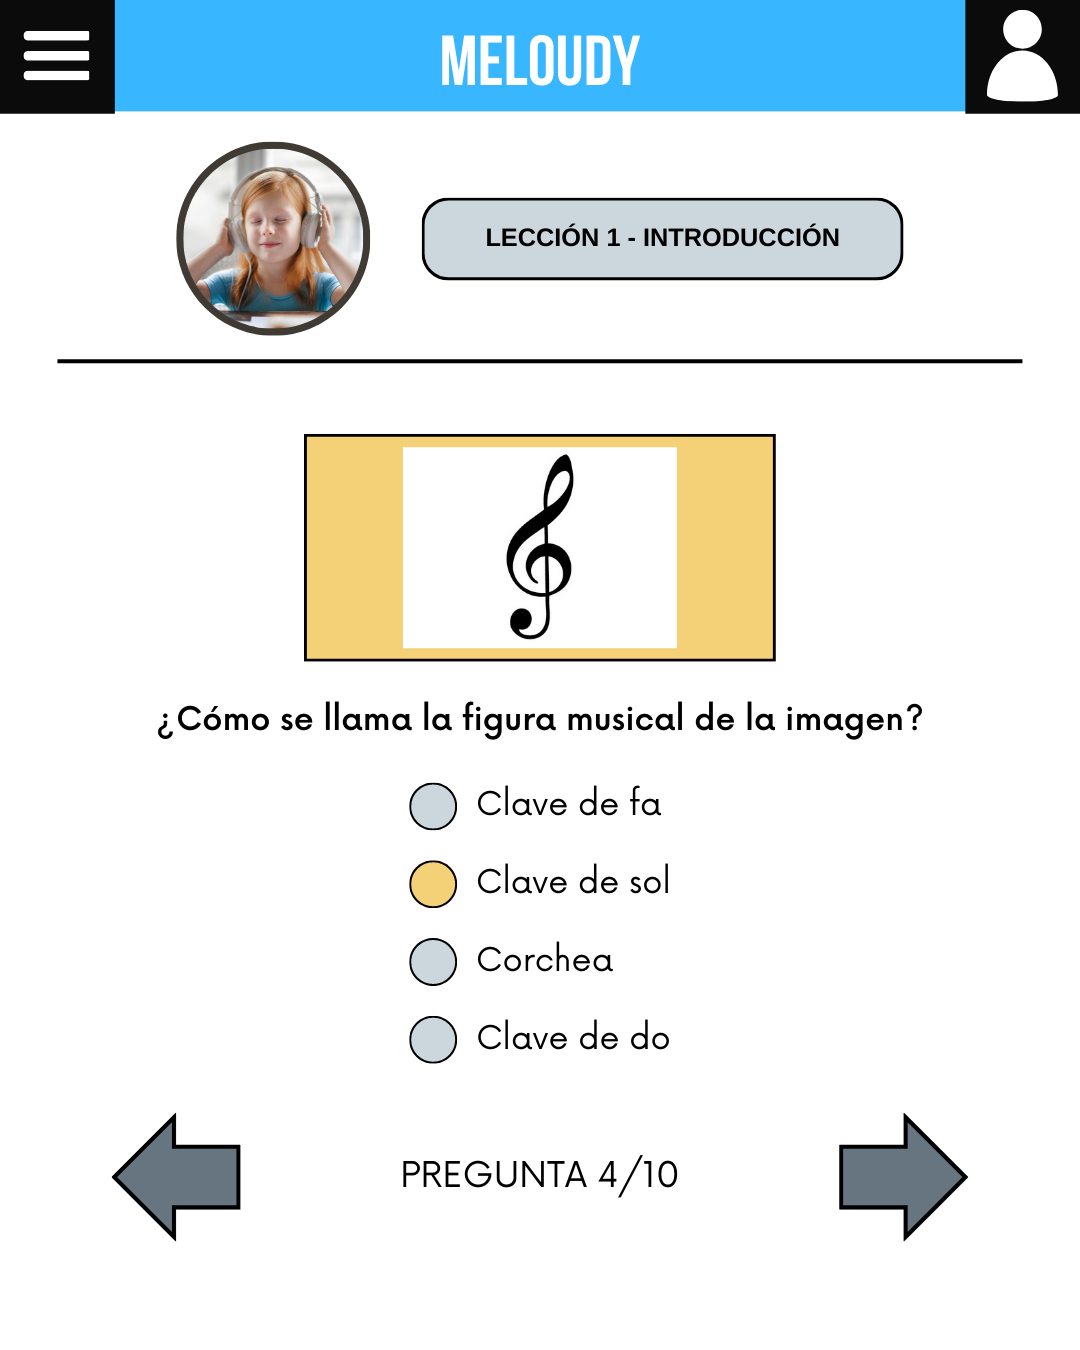
\includegraphics[width=0.45\textwidth, frame]{imagenes/c6/5.png}}
    \caption{Boceto de la pantalla de una pregunta de test de tipo selección única.}
    \label{fig:seleccionunica}
\end{figure}

\newpage

\subsection*{Pregunta de selección múltiple}

Con esta vista se mostrará al usuario una pregunta de test de tipo selección múltiple. En ella se mostrará la pregunta y las opciones de respuesta. El usuario podrá seleccionar todas las opciones que considere correctas y pulsar en el botón de comprobar para comprobar si las respuestas son correctas o no. Si las respuestas son correctas, se mostrará un mensaje de felicitación y se mostrará el botón de siguiente para pasar a la siguiente pregunta. Si las respuestas son incorrectas, se mostrará un mensaje de error y se mostrará el botón de siguiente para pasar a la siguiente pregunta. Si el usuario no ha seleccionado ninguna opción, se mostrará un mensaje de error y no se podrá pasar a la siguiente pregunta hasta que no seleccione una opción.

\begin{figure}[H]
    \centering
    \centerline{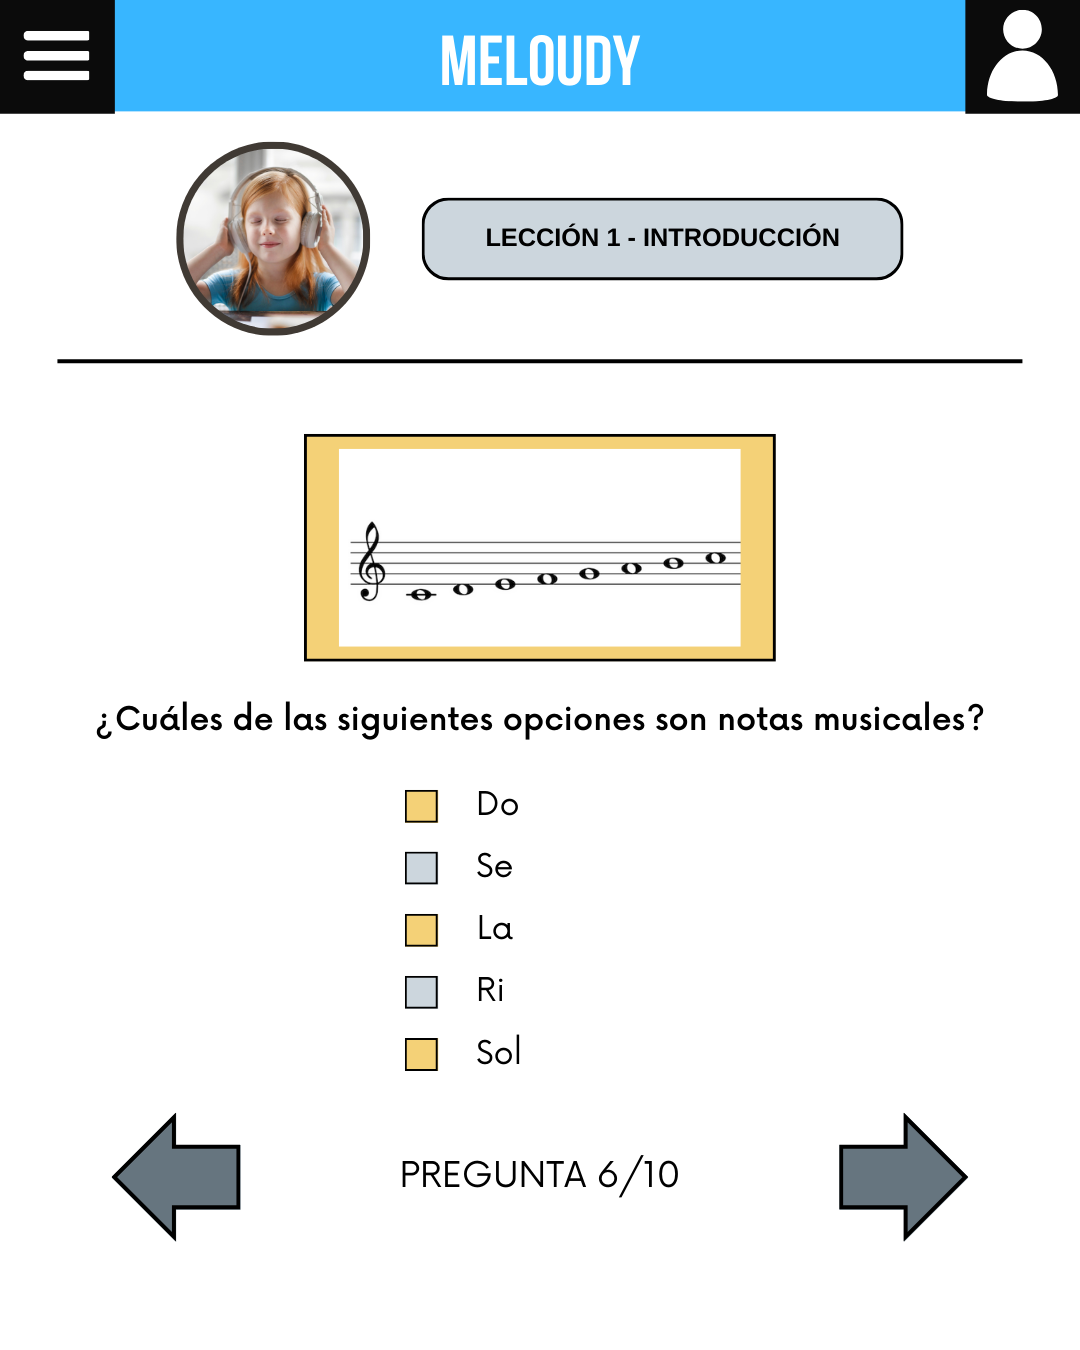
\includegraphics[width=0.55\textwidth, frame]{imagenes/c6/6.png}}
    \caption{Boceto de la pantalla de una pregunta de test de tipo selección multiple.}
    \label{fig:seleccionmultiple}
\end{figure}

\newpage

\subsection*{Pregunta de escritura de texto}

Con esta vista se mostrará al usuario una pregunta de test de tipo escritura de texto. En ella se mostrará la pregunta y el usuario deberá escribir la respuesta en el campo de texto. El usuario podrá pulsar en el botón de comprobar para comprobar si la respuesta es correcta o no. Si la respuesta es correcta, se mostrará un mensaje de felicitación y se mostrará el botón de siguiente para pasar a la siguiente pregunta. Si la respuesta es incorrecta, se mostrará un mensaje de error y se mostrará el botón de siguiente para pasar a la siguiente pregunta. Si el usuario no ha escrito ninguna respuesta, se mostrará un mensaje de error y no se podrá pasar a la siguiente pregunta hasta que no escriba una respuesta.

\begin{figure}[H]
    \centering
    \centerline{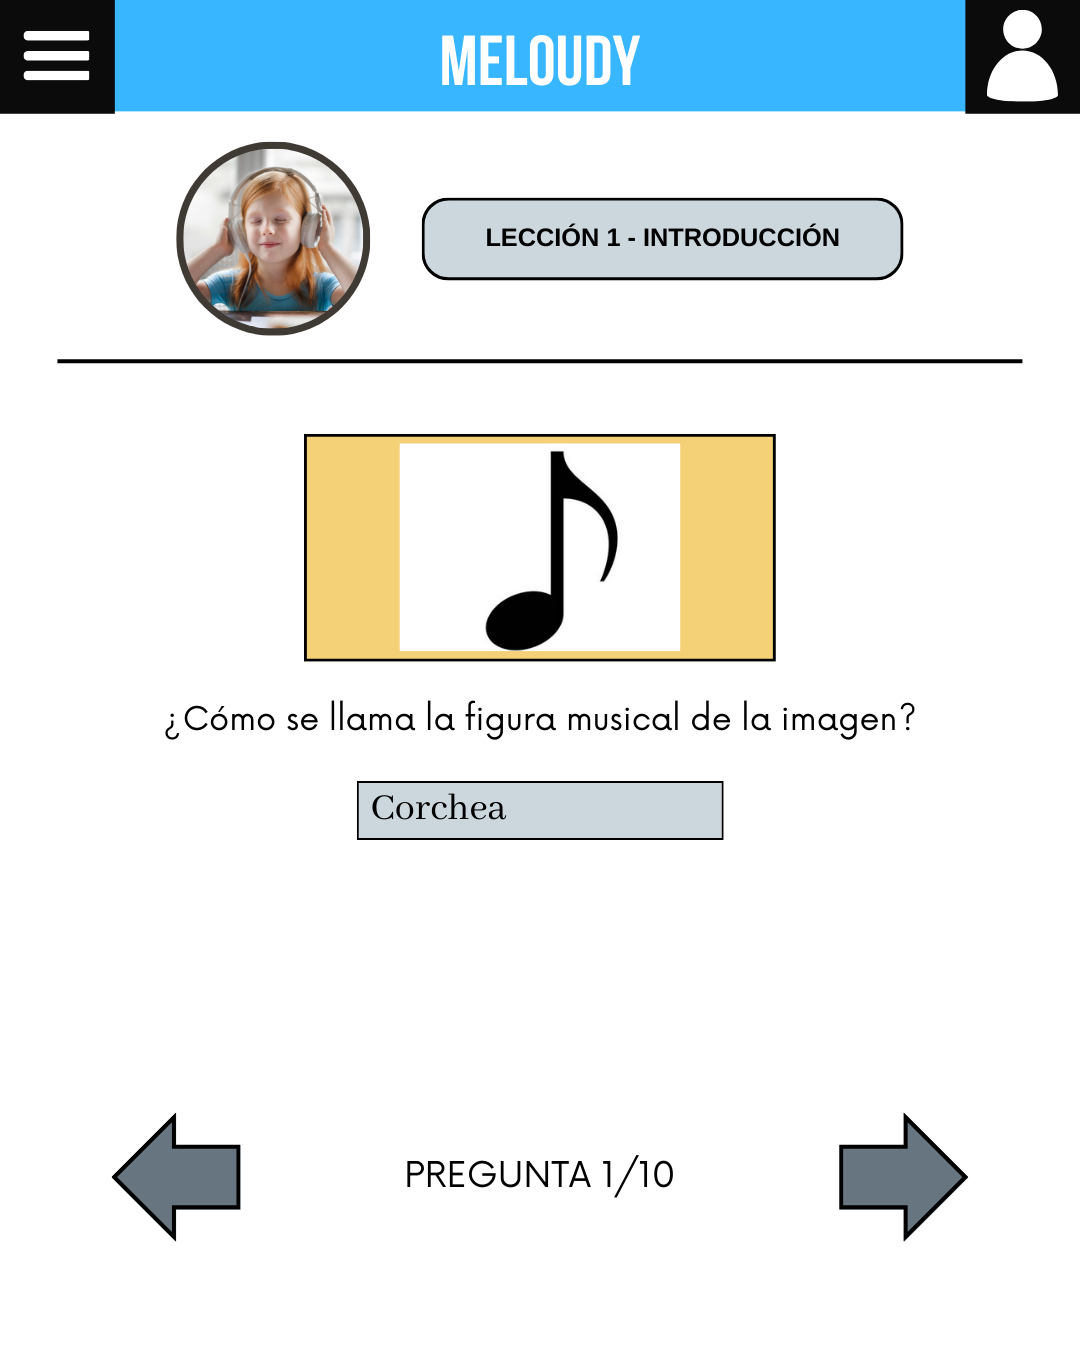
\includegraphics[width=0.55\textwidth, frame]{imagenes/c6/7.png}}
    \caption{Boceto de la pantalla de una pregunta de test de tipo escritura de texto.}
    \label{fig:escrituratexto}
\end{figure}

\newpage

\subsection*{Pregunta de entrada por micrófono}

Con esta vista se mostrará al usuario una pregunta de test de tipo entrada por micrófono. En ella se mostrará la pregunta y el usuario deberá pulsar en el botón de grabar para grabar la respuesta, que deberá ser la melodia que pida la pregunta. El usuario podrá pulsar en el botón de comprobar para comprobar si la respuesta es correcta o no. Si la respuesta es correcta, se mostrará un mensaje de felicitación y se mostrará el botón de siguiente para pasar a la siguiente pregunta. Si la respuesta es incorrecta, se mostrará un mensaje de error y se mostrará el botón de siguiente para pasar a la siguiente pregunta. Si el usuario no ha grabado ninguna respuesta, se mostrará un mensaje de error y no se podrá pasar a la siguiente pregunta hasta que no grabe una respuesta.

\begin{figure}[H]
    \centering
    \centerline{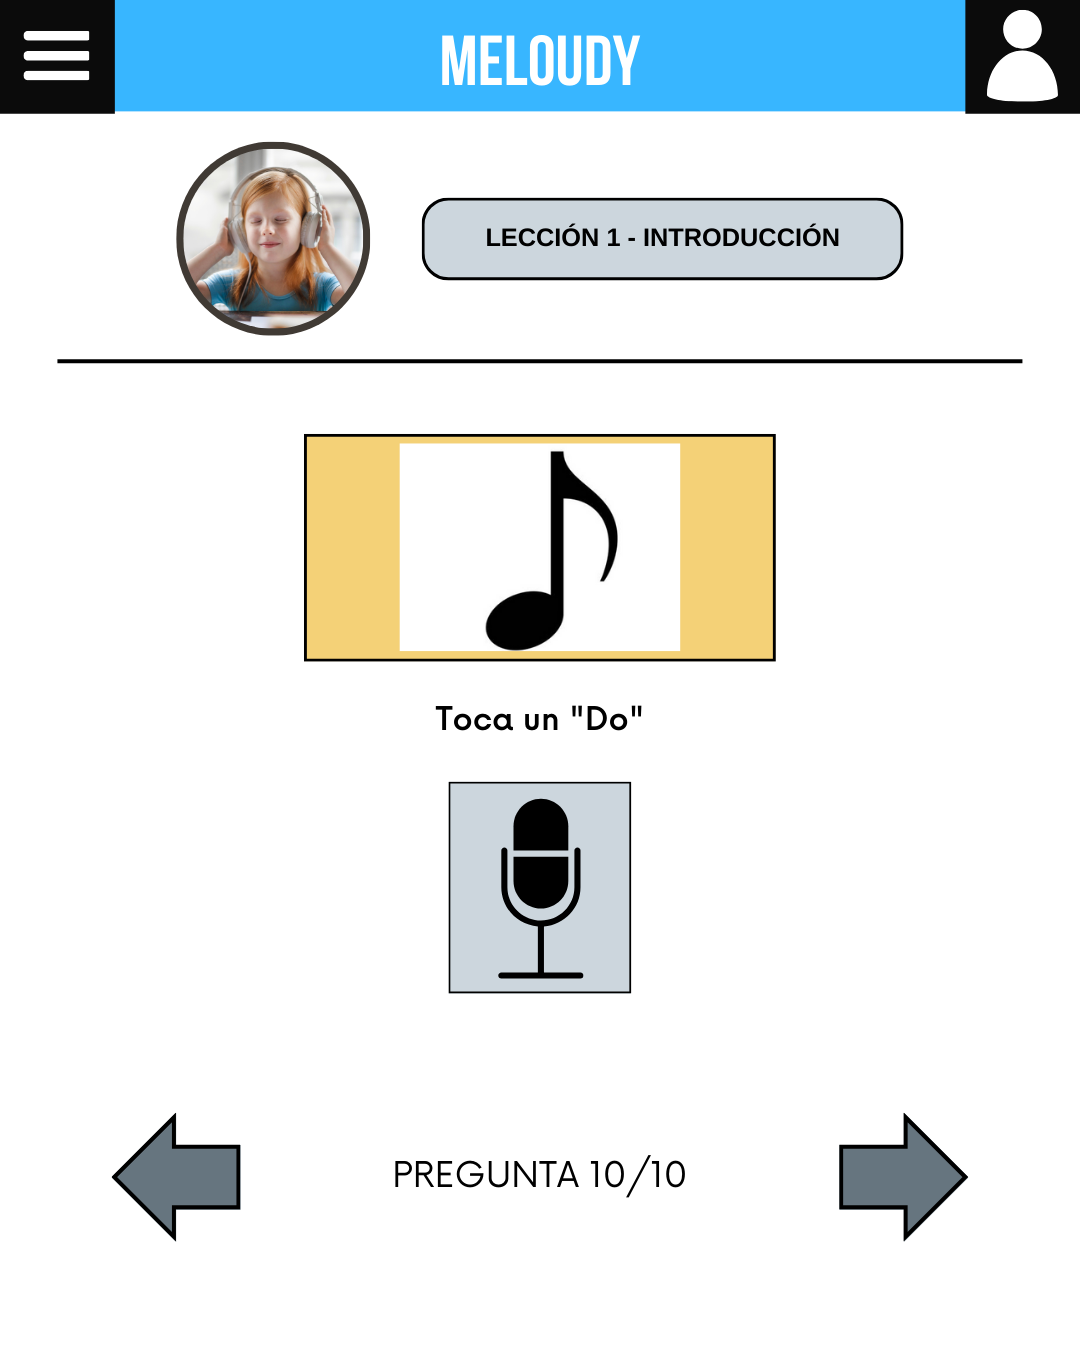
\includegraphics[width=0.55\textwidth, frame]{imagenes/c6/8.png}}
    \caption{Boceto de la pantalla de una pregunta de test de tipo entrada por micrófono.}
    \label{fig:microfono}
\end{figure}

\newpage

\subsection*{Diagrama de navegación}

Para finalizar la sección se presenta un diagrama de navegación de la aplicación, el cual muestra las distintas pantallas que tendrá la aplicación siguiendo el flujo que un usuario tendría al utilizar la aplicación.
\begin{figure}[H]
    \centering
    \centerline{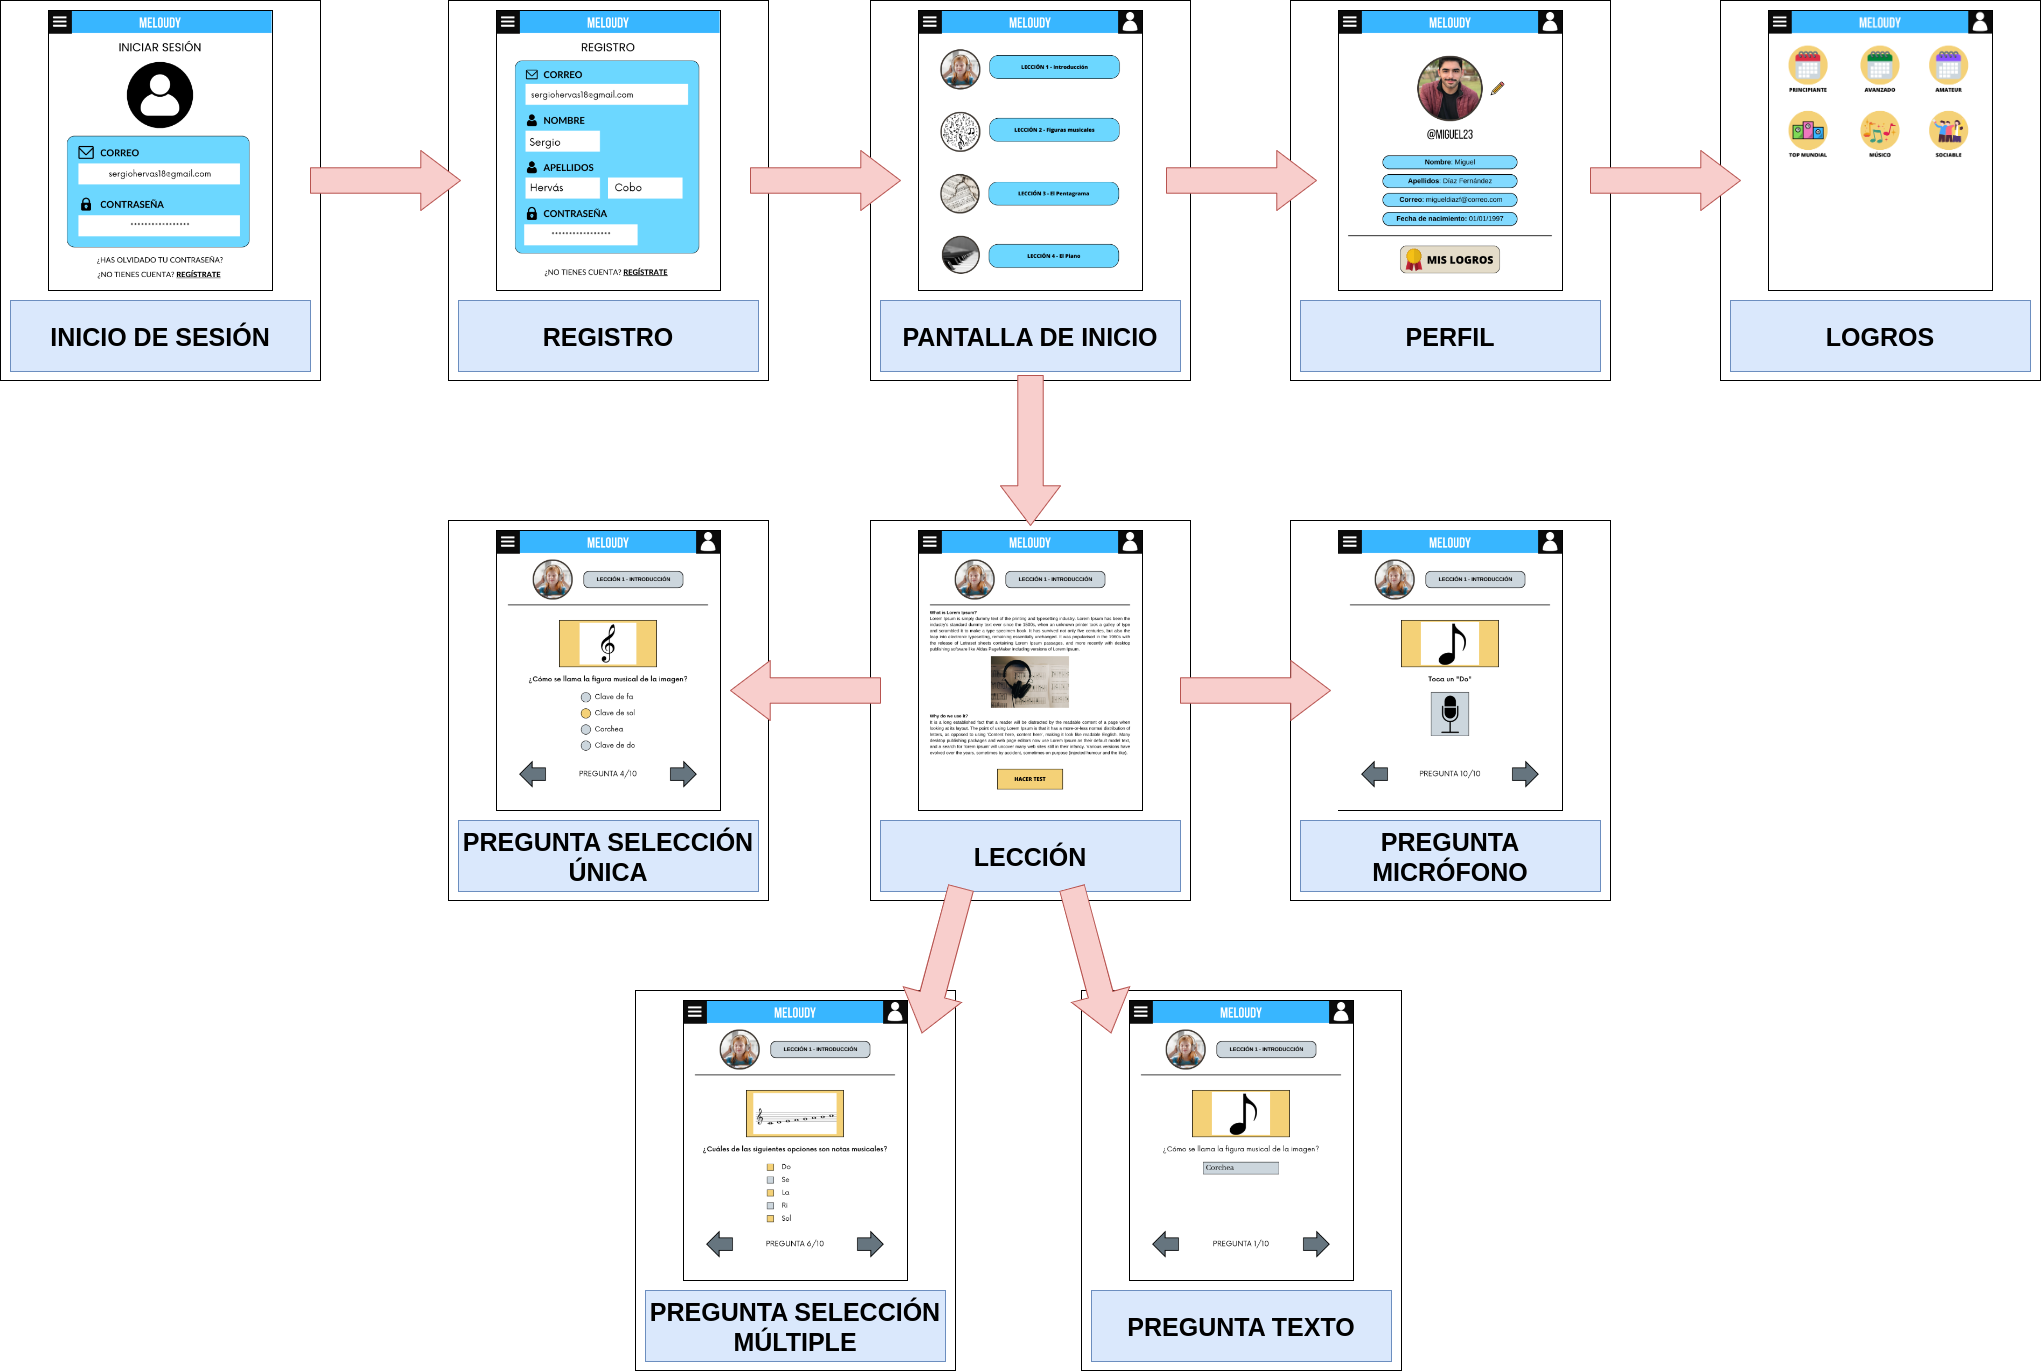
\includegraphics[width=1.2\textwidth]{imagenes/c6/diagrambocetos.png}}
    \caption{Diagrama de navegación de la aplicación por los distintos bocetos presentados anteriormente que muestra las pantallas que seguirá el usuario cuando utilice la aplicación.}
    \label{fig:microfono}
\end{figure}

